\begin{frame}{Discrete Time Sequence}

From \structure{scalar} sequence $u_{1}, \ldots, u_L$ to $y_1, \ldots, y_L$.

\begin{figure}
    \centering
    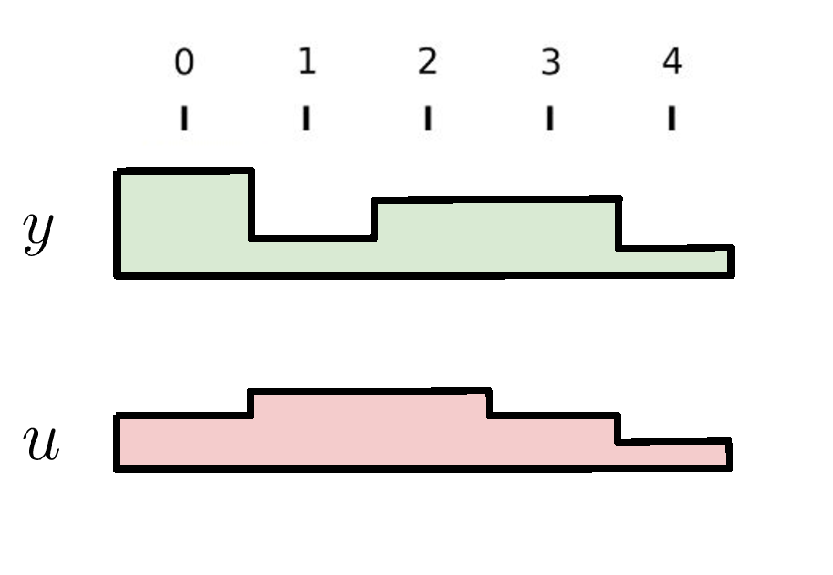
\includegraphics[width=0.5\textwidth]{Figs/SSMStart.pdf}
    \label{fig:my_label}
\end{figure}
\end{frame}


\begin{frame}{Review: RNN for Language Generation}
    \begin{columns}
    \begin{column}{0.5\textwidth}
        \centering
              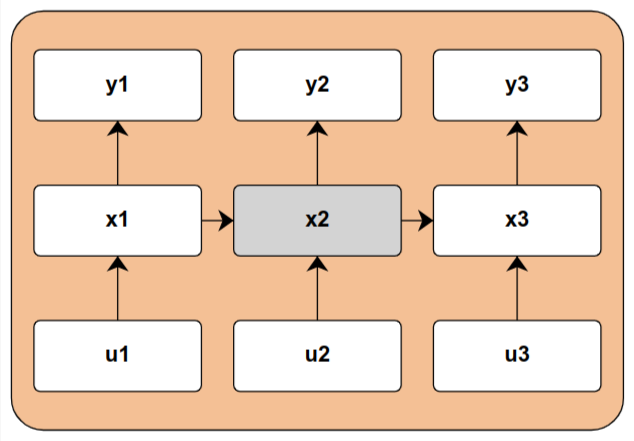
\includegraphics[width=.8\textwidth]{Figs/rnn.png}

    \end{column}
    \begin{column}{0.5\textwidth}

    \begin{align*}
    x_{k} &= \textcolor{red}{\sigma}(\textcolor{green}{\boldsymbol{\overline{A}}} x_{k-1} + \textcolor{blue}{\boldsymbol{\overline{B}}} u_k) \\ 
    y_k &= \phantom{\sigma (} \textcolor{orange}{\boldsymbol{\overline{C}}} x_{k \phantom{- 1}}
    \end{align*}
    \end{column}
    \end{columns}

\end{frame}

\begin{frame}{Review: RNN versus Attention}
    \begin{columns}
    \begin{column}{0.5\textwidth}
        \centering
        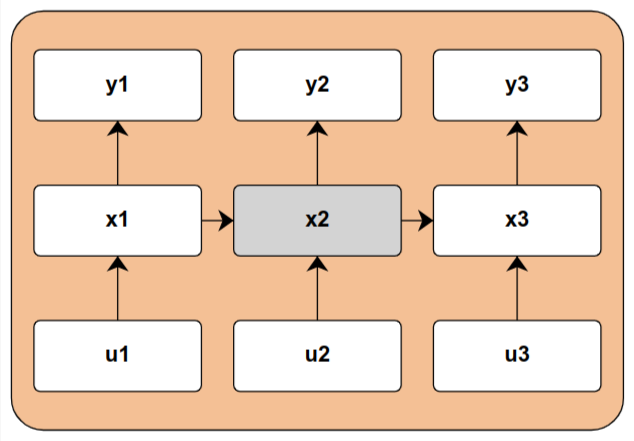
\includegraphics[width=.8\textwidth]{Figs/rnn.png}
    \end{column}
    \begin{column}{0.5\textwidth}
        \centering
  
        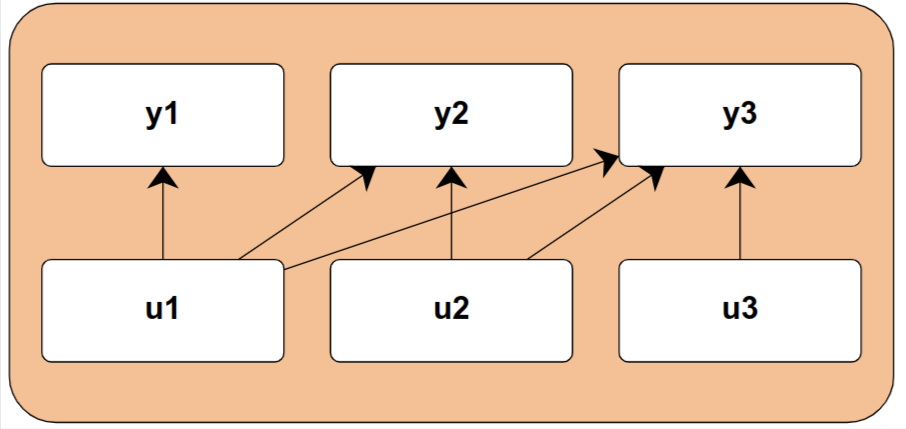
\includegraphics[width=0.8\textwidth]{Figs/out5.png}
    \end{column}
    \end{columns}
    \vspace{0.5cm}
    
\begin{itemize}
    \item \structure{Training Speed:} Slow (\textcolor{red}{Serial} bottleneck)
    \item \structure{Generation Speed:} Fast (constant-time per step)
    
\end{itemize}
\end{frame}


\begin{frame}{Didn't we try this RNN thing?  }

\begin{center}    
The last major RNN model in NLP - \textcolor{red}{ELMo}
\end{center}

\pause

    \begin{figure}
        \centering
        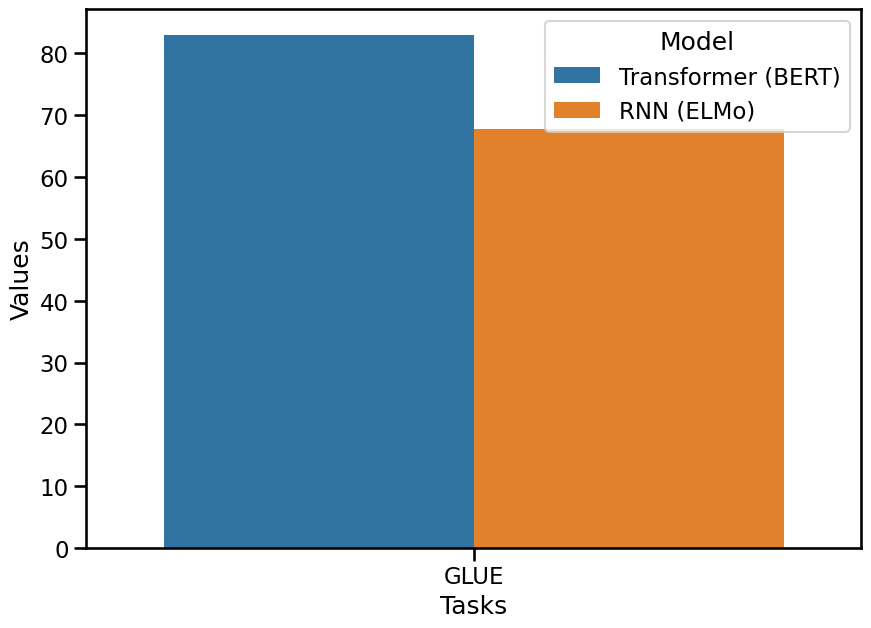
\includegraphics[width=0.5\textwidth]{Figs/GLUE.png}

        \label{fig:my_label}
    \end{figure}
\blfootnote{\cite{DBLP:conf/naacl/PetersNIGCLZ18, devlin2018bert}}
\end{frame}

\begin{frame}{RNN Revival: Two Differences}
\begin{columns}
    \begin{column}{0.5\textwidth}
        
    \begin{enumerate}
        \item Efficient Linear RNNs
        \item Effective Long-Range Parameterizations
    \end{enumerate}

    
    % Orthogonal RNN - Linear 
    % QRNN - > Linear RNN. $\bar{A}$ time-varying Linear non-homogenous. input depdendent 

    % A static over time. 
    % SISO - property. 
    % Orthogonal - > 
    
    \end{column}
    \begin{column}{0.5\textwidth}
\centering
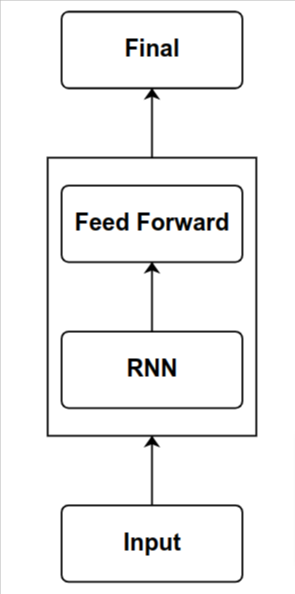
\includegraphics[width=0.4\textwidth, clip,trim={0.1cm 0.1cm 0.1cm 0.1cm}]{Figs/out-rnn.png}
    \end{column}

\end{columns}
\end{frame}



\begin{frame}{Component 1: \textcolor{blue}{Linear} RNN}

    \begin{align*}
    x_{k} &= \textcolor{green}{\boldsymbol{\overline{A}}} \textcolor{black}{\boldsymbol{x}_{k-1}} + \textcolor{blue}{\boldsymbol{\overline{B}}} \textcolor{black}{u_k} \\ 
    y_k &=  \textcolor{orange}{\boldsymbol{\overline{C}}} x_{k \phantom{- 1}}
    \end{align*}
    \pause
    \begin{figure}
        \centering
        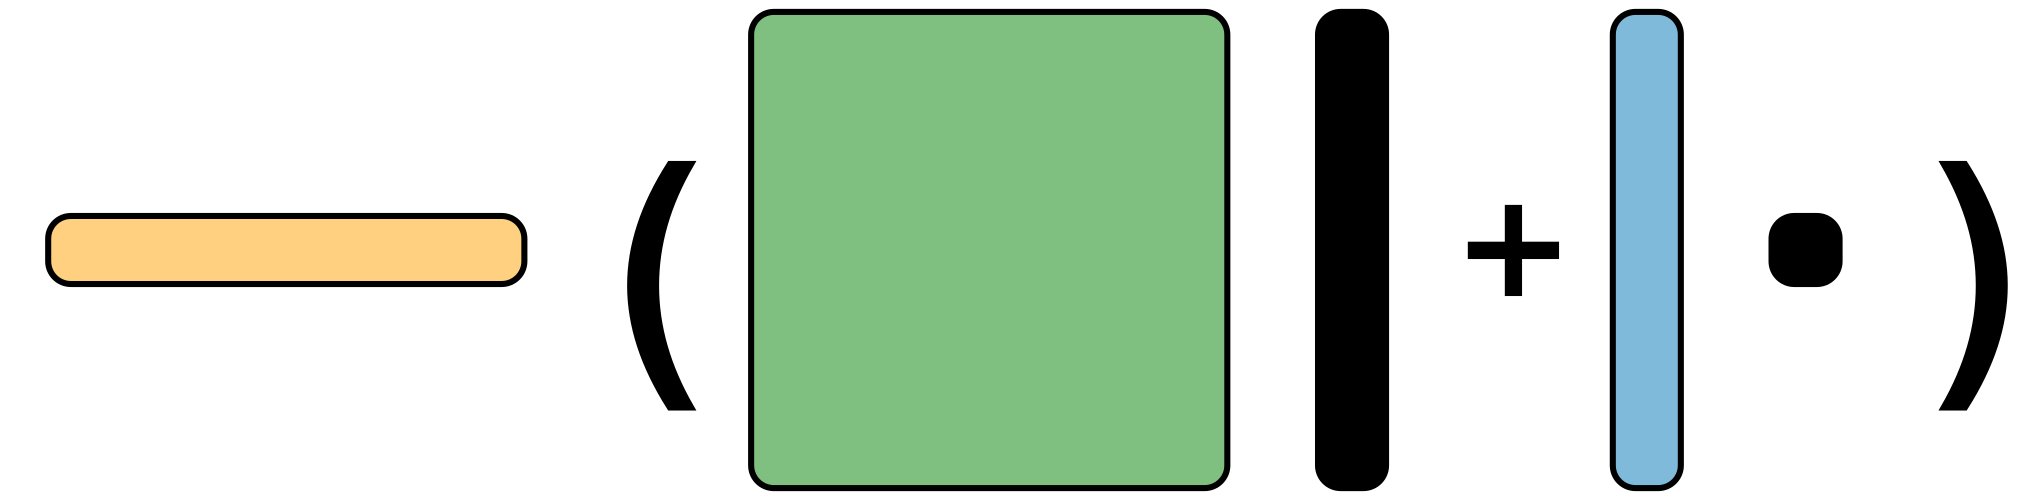
\includegraphics[width=0.6\textwidth]{Figs/ssm.png}
        \label{fig:my_label}
    \end{figure}
\end{frame}

\begin{frame}{Expansion Of Terms}
\vspace{-0.5cm}
    \begin{align*}
    y_k =  \textcolor{orange}{\boldsymbol{\overline{C}}} x_{k \phantom{- 1}} \ 
    x_{k} = \textcolor{green}{\boldsymbol{\overline{A}}} \textcolor{black}{\boldsymbol{x}_{k-1}} + \textcolor{blue}{\boldsymbol{\overline{B}}} \textcolor{black}{u_k} \ 
    \end{align*}
    \pause 
    \vspace{-2cm}
\begin{figure}
    \centering
    \only<2>{\[y_1\]}\only<3>{\[y_2\]} \only<4->{\[y_3\]}
    \includegraphics<2>[height=0.12\textwidth]{Figs/ssmrec0}
    
    \includegraphics<3>[height=0.12\textwidth]{Figs/ssmrec1}
    
     \includegraphics<4->[height=0.1\textwidth]{Figs/ssmrec}
    \label{fig:my_label}
\end{figure}
\vspace{-0.5cm}

\pause\pause\pause
\begin{align*}
\overline{K} &= (\textcolor{orange}{\boldsymbol{\overline{C}}}\textcolor{blue}{\boldsymbol{\overline{B}}}, \textcolor{orange}{\boldsymbol{\overline{C}}}\textcolor{green}{\boldsymbol{\overline{A}}}\textcolor{blue}{\boldsymbol{\overline{B}}}, \dots, \textcolor{orange}{\boldsymbol{\overline{C}}}\textcolor{green}{\boldsymbol{\overline{A}}^{L-1}}\textcolor{blue}{\boldsymbol{\overline{B}}})
\end{align*}
\end{frame}

\begin{frame}{Convolutional Form}

    \begin{align*}
    y_k =  \textcolor{orange}{\boldsymbol{\overline{C}}} x_{k \phantom{- 1}} \ 
    x_{k} = \textcolor{green}{\boldsymbol{\overline{A}}} \textcolor{black}{\boldsymbol{x}_{k-1}} + \textcolor{blue}{\boldsymbol{\overline{B}}} \textcolor{black}{u_k} \ 
    \end{align*}



\begin{align*}
\overline{K} &= (\textcolor{orange}{\boldsymbol{\overline{C}}}\textcolor{blue}{\boldsymbol{\overline{B}}}, \textcolor{orange}{\boldsymbol{\overline{C}}}\textcolor{green}{\boldsymbol{\overline{A}}}\textcolor{blue}{\boldsymbol{\overline{B}}}, \dots, \textcolor{orange}{\boldsymbol{\overline{C}}}\textcolor{green}{\boldsymbol{\overline{A}}^{L-1}}\textcolor{blue}{\boldsymbol{\overline{B}}}) \\
y &= \text{conv1d}(\overline{K}_L \ldots \overline{K}_1, u_1 \ldots u_L)
\end{align*}



% Intuition: 
% \pause
% $$y_1 = \boldsymbol{\overline{C}} \boldsymbol{\overline{B}} u_1$$ 
% \pause
% $$y_2 = \boldsymbol{\overline{C}} \boldsymbol{\overline{A}} \boldsymbol{\overline{B}} u_1 + \boldsymbol{\overline{C}} \boldsymbol{\overline{B}} u_2 = \boldsymbol{\overline{C}} (\boldsymbol{\overline{A}} \boldsymbol{\overline{B}} u_1 + \boldsymbol{\overline{B}} u_2) = \boldsymbol{\overline{C}} (\boldsymbol{x}_1 + \boldsymbol{\overline{B}} u_2) $$
\end{frame}


\begin{frame}{Convolutional Form}
\begin{align*}
\overline{K} &= (\textcolor{black}{\boldsymbol{\overline{C}}}\textcolor{black}{\boldsymbol{\overline{B}}}, \textcolor{black}{\boldsymbol{\overline{C}}}\textcolor{black}{\boldsymbol{\overline{A}}}\textcolor{black}{\boldsymbol{\overline{B}}}, \dots, \textcolor{black}{\boldsymbol{\overline{C}}}\textcolor{black}{\boldsymbol{\overline{A}}^{L-1}}\textcolor{black}{\boldsymbol{\overline{B}}}) \\
\end{align*}
\begin{figure}
    \centering
    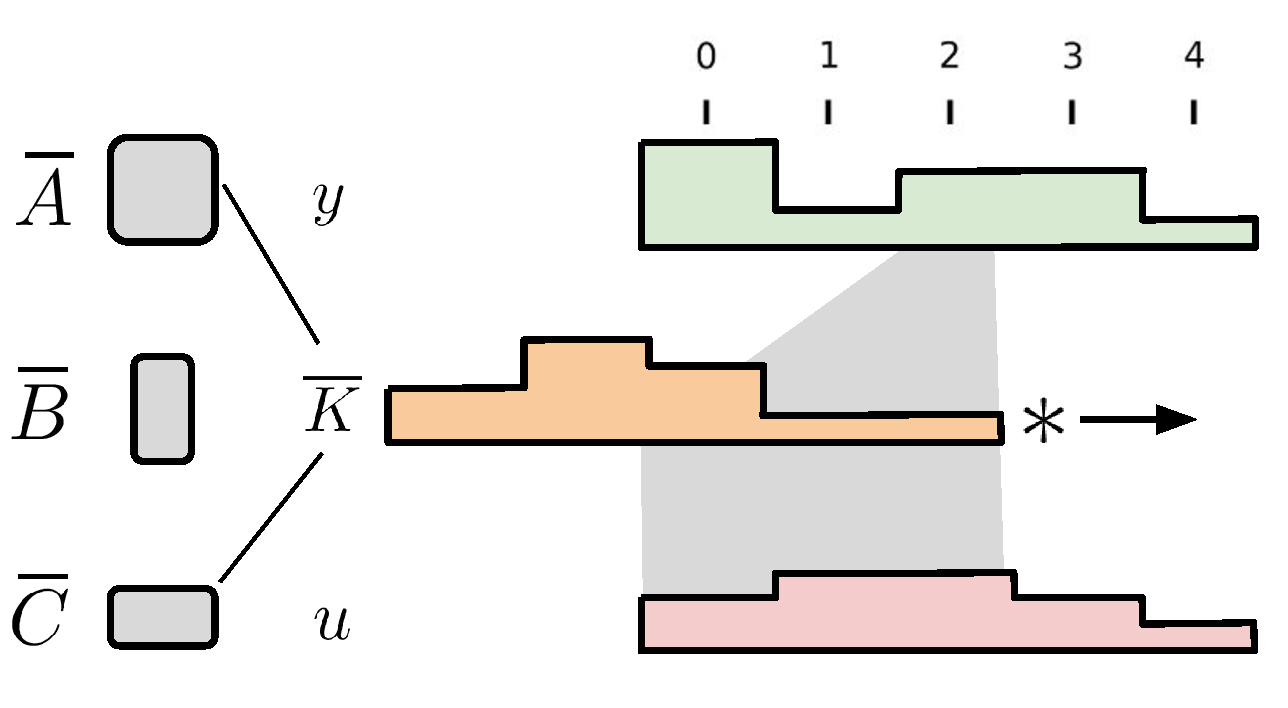
\includegraphics[width=0.6\textwidth]{Figs/SSM (1).pdf}
    \label{fig:my_label}
\end{figure}
\end{frame}

\begin{frame}{Computation 1: FFT}
Compute convolution in Fourier space, 

\begin{align*}
&y = \boldsymbol{\overline{K}} \ast u
\end{align*}
\begin{itemize}
    \item $O(L \log L)$ for padded FFT of $K$ and $u$, mult, then iFFT
    \item Accelerators optimize this to different levels.
\end{itemize}
\end{frame}

\begin{frame}[c]{Computation 2: Associative Scan (S5)}


\begin{columns}
    \begin{column}{0.5\textwidth}
    Associative $e_1\bullet \ldots \bullet e_L$

    \begin{center}
    \Tree [.$\bullet$ [.$\bullet$ [.$\bullet$ $e_1$ ] [.$\bullet$ $e_2$ ] ] [.$\bullet$ [.$\bullet$ $e_3$ ] [.$\bullet$ $e_4$ ] ] ]
    \end{center}
    \end{column}
        
 \begin{column}{0.5\textwidth}
 \centering
 \[e_k = (\boldsymbol{E}_k, \boldsymbol{e}_k) = (\bar{\textcolor{green}{\boldsymbol{A}}}, \bar{\textcolor{blue}{\boldsymbol{B}}}u_k)\]
    \begin{figure}
        \centering
        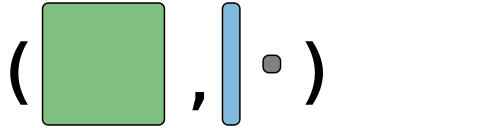
\includegraphics[height=0.1\textwidth,clip,trim={0cm 0cm 6cm 0cm}]{Figs/assoc.png}
        \label{fig:my_label}
    \end{figure}
    \[e_i \bullet e_j = (\boldsymbol{E}_i \boldsymbol{E}_j, \boldsymbol{E}_j \boldsymbol{e}_i + \boldsymbol{e}_j ) \]
    \begin{figure}
        \centering
        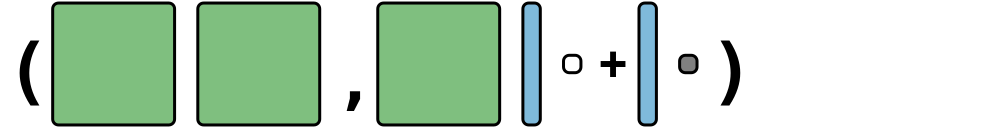
\includegraphics[height=0.1\textwidth,clip,trim={0cm 0cm 6cm 0cm}]{Figs/assoc2.png}
    \end{figure}
        
    \end{column}
\end{columns}
    \blfootnote{\cite{Blelloch1990-yo,Martin2018-bq,smith2022simplified}}
\end{frame}
% \begin{frame}{Alternative Computation: Associative Scan \cite{smith2022simplified}}
   

% \end{frame}


% \begin{frame}{ Associative Scan: S5 }
%     Potential benefits versus FFT
%     \vspace{0.5cm}
    
%     \begin{itemize}
%         \item Compute hidden states explicitly
%         \item Allows alternative RNN forms.
%         \item Faster on some architectures
%     \end{itemize}
% \end{frame}


\begin{frame}{Linear RNN Computational Profile}

    \begin{align*}
    x_{k} &= \textcolor{green}{\boldsymbol{\overline{A}}} \textcolor{black}{{x}_{k-1}} + \textcolor{blue}{\boldsymbol{\overline{B}}} \textcolor{black}{u_k} \\ 
    y_k &=  \textcolor{orange}{\boldsymbol{\overline{C}}} x_{k \phantom{- 1}}
    \end{align*}
\begin{itemize}
    \item \structure{Training Speed:} \sout{Weak} Strong (Parallelizable convolution)
    \item \structure{Generation Speed:} Strong (constant-time per step) \pause
    \item \structure{Accuracy:} Extremely \textcolor{red}{Poor...} Barely learns.
\end{itemize}
\end{frame}

\begin{frame}{Interactions}
    \begin{center}
        Routing here must be static and regular (conv). 
    \end{center}
    \begin{figure}
        \centering
        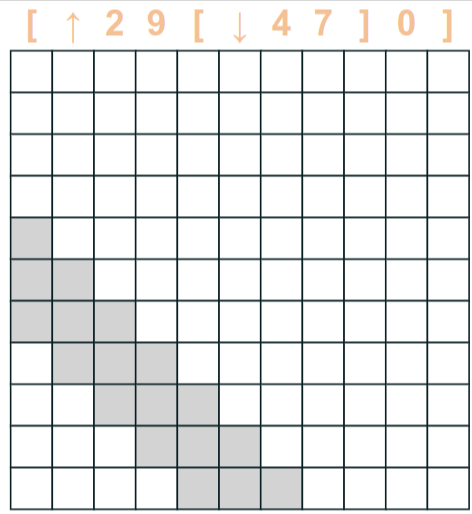
\includegraphics[height=0.45\textheight,clip,trim={0.1cm 0.1cm 0.1cm 0.1cm}]{Figs/Allowed.png}
        \vspace{0.5cm}
        
        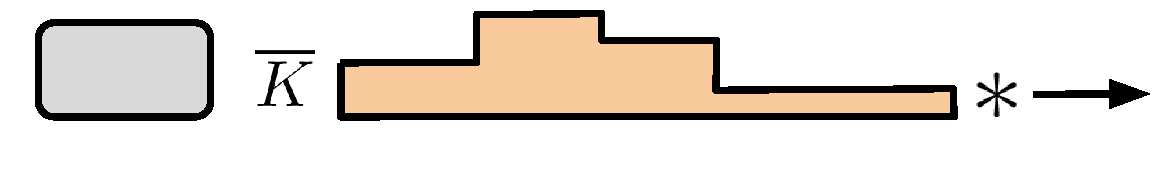
\includegraphics[width=0.5\textwidth]{Figs/SGParam.pdf}
        \label{fig:my_label}
    \end{figure}
\end{frame}




\begin{frame}{Component 2:  Model Parameterization}

Linear RNN behavior highly dependent on $\boldsymbol{\overline{A}}$

\begin{align*}
\overline{K} &= (\textcolor{orange}{\boldsymbol{\overline{C}}}\textcolor{blue}{\boldsymbol{\overline{B}}}, \textcolor{orange}{\boldsymbol{\overline{C}}}\textcolor{green}{\boldsymbol{\overline{A}}}\textcolor{blue}{\boldsymbol{\overline{B}}}, \dots, \textcolor{orange}{\boldsymbol{\overline{C}}}\textcolor{green}{\boldsymbol{\overline{A}}^{L-1}}\textcolor{blue}{\boldsymbol{\overline{B}}})
\end{align*}
\vspace{0.5cm}

Choice of $\boldsymbol{\overline{A}}$ is critical: stable and informative.
\end{frame}


\begin{frame}{Mathematical Model: State Space Model (SSM) }

A SSM is a continuous-time, differential equation.
\begin{align*}
    x'(t) &= \boldsymbol{A}x(t) + \boldsymbol{B}u(t) \\  
    y(t) &= \boldsymbol{C}x(t).
\end{align*}

Used to explore Linear RNN parameterization.
\end{frame}

\begin{frame}{Hidden State Form~\cite{gu2020hippo}}
  \textcolor{red}{Summarize} history in vector $x$ with \textcolor{blue}{Legendre} coefficients 
    \begin{figure}
    \centering
    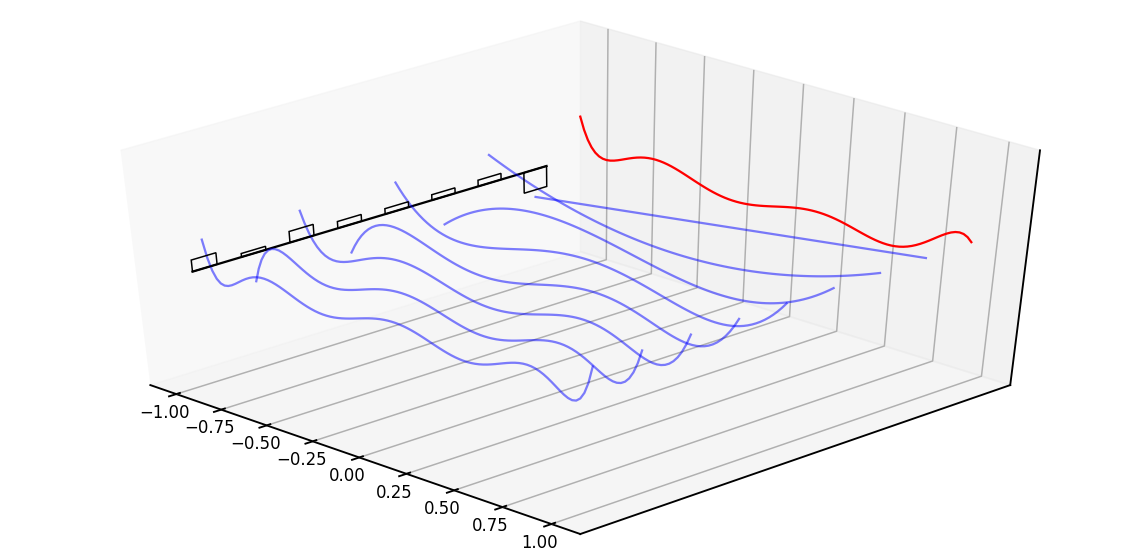
\includegraphics[width=0.7\textwidth]{Figs/hippo.png}
    \end{figure}
\end{frame}

\begin{frame}{Choice of Parameters~\cite{gu2020hippo}}
    Intuition: Hidden state vector $\textcolor{blue}{x}$ should \textcolor{red}{summarize} past $u$. 

\begin{figure}
    \centering
    \includegraphics<1>[width=\textwidth]{Figs/frame_10_delay-0.1s.png}
    \includegraphics<2>[width=\textwidth]{Figs/frame_20_delay-0.1s.png}
    \includegraphics<3>[width=\textwidth]{Figs/frame_30_delay-0.1s.png}
    \includegraphics<4>[width=1\textwidth]{Figs/frame_40_delay-0.1s.png}
    \includegraphics<5>[width=1\textwidth]{Figs/frame_50_delay-0.1s.png}
\end{figure}

\end{frame}



% \begin{frame}{Practical Consequence: HiPPO~\cite{gu2020hippo}}
%     Motivates an initialization of the (discrete-time) kernel $\bar{K}$.
    
%     \begin{figure}
%         \centering
%         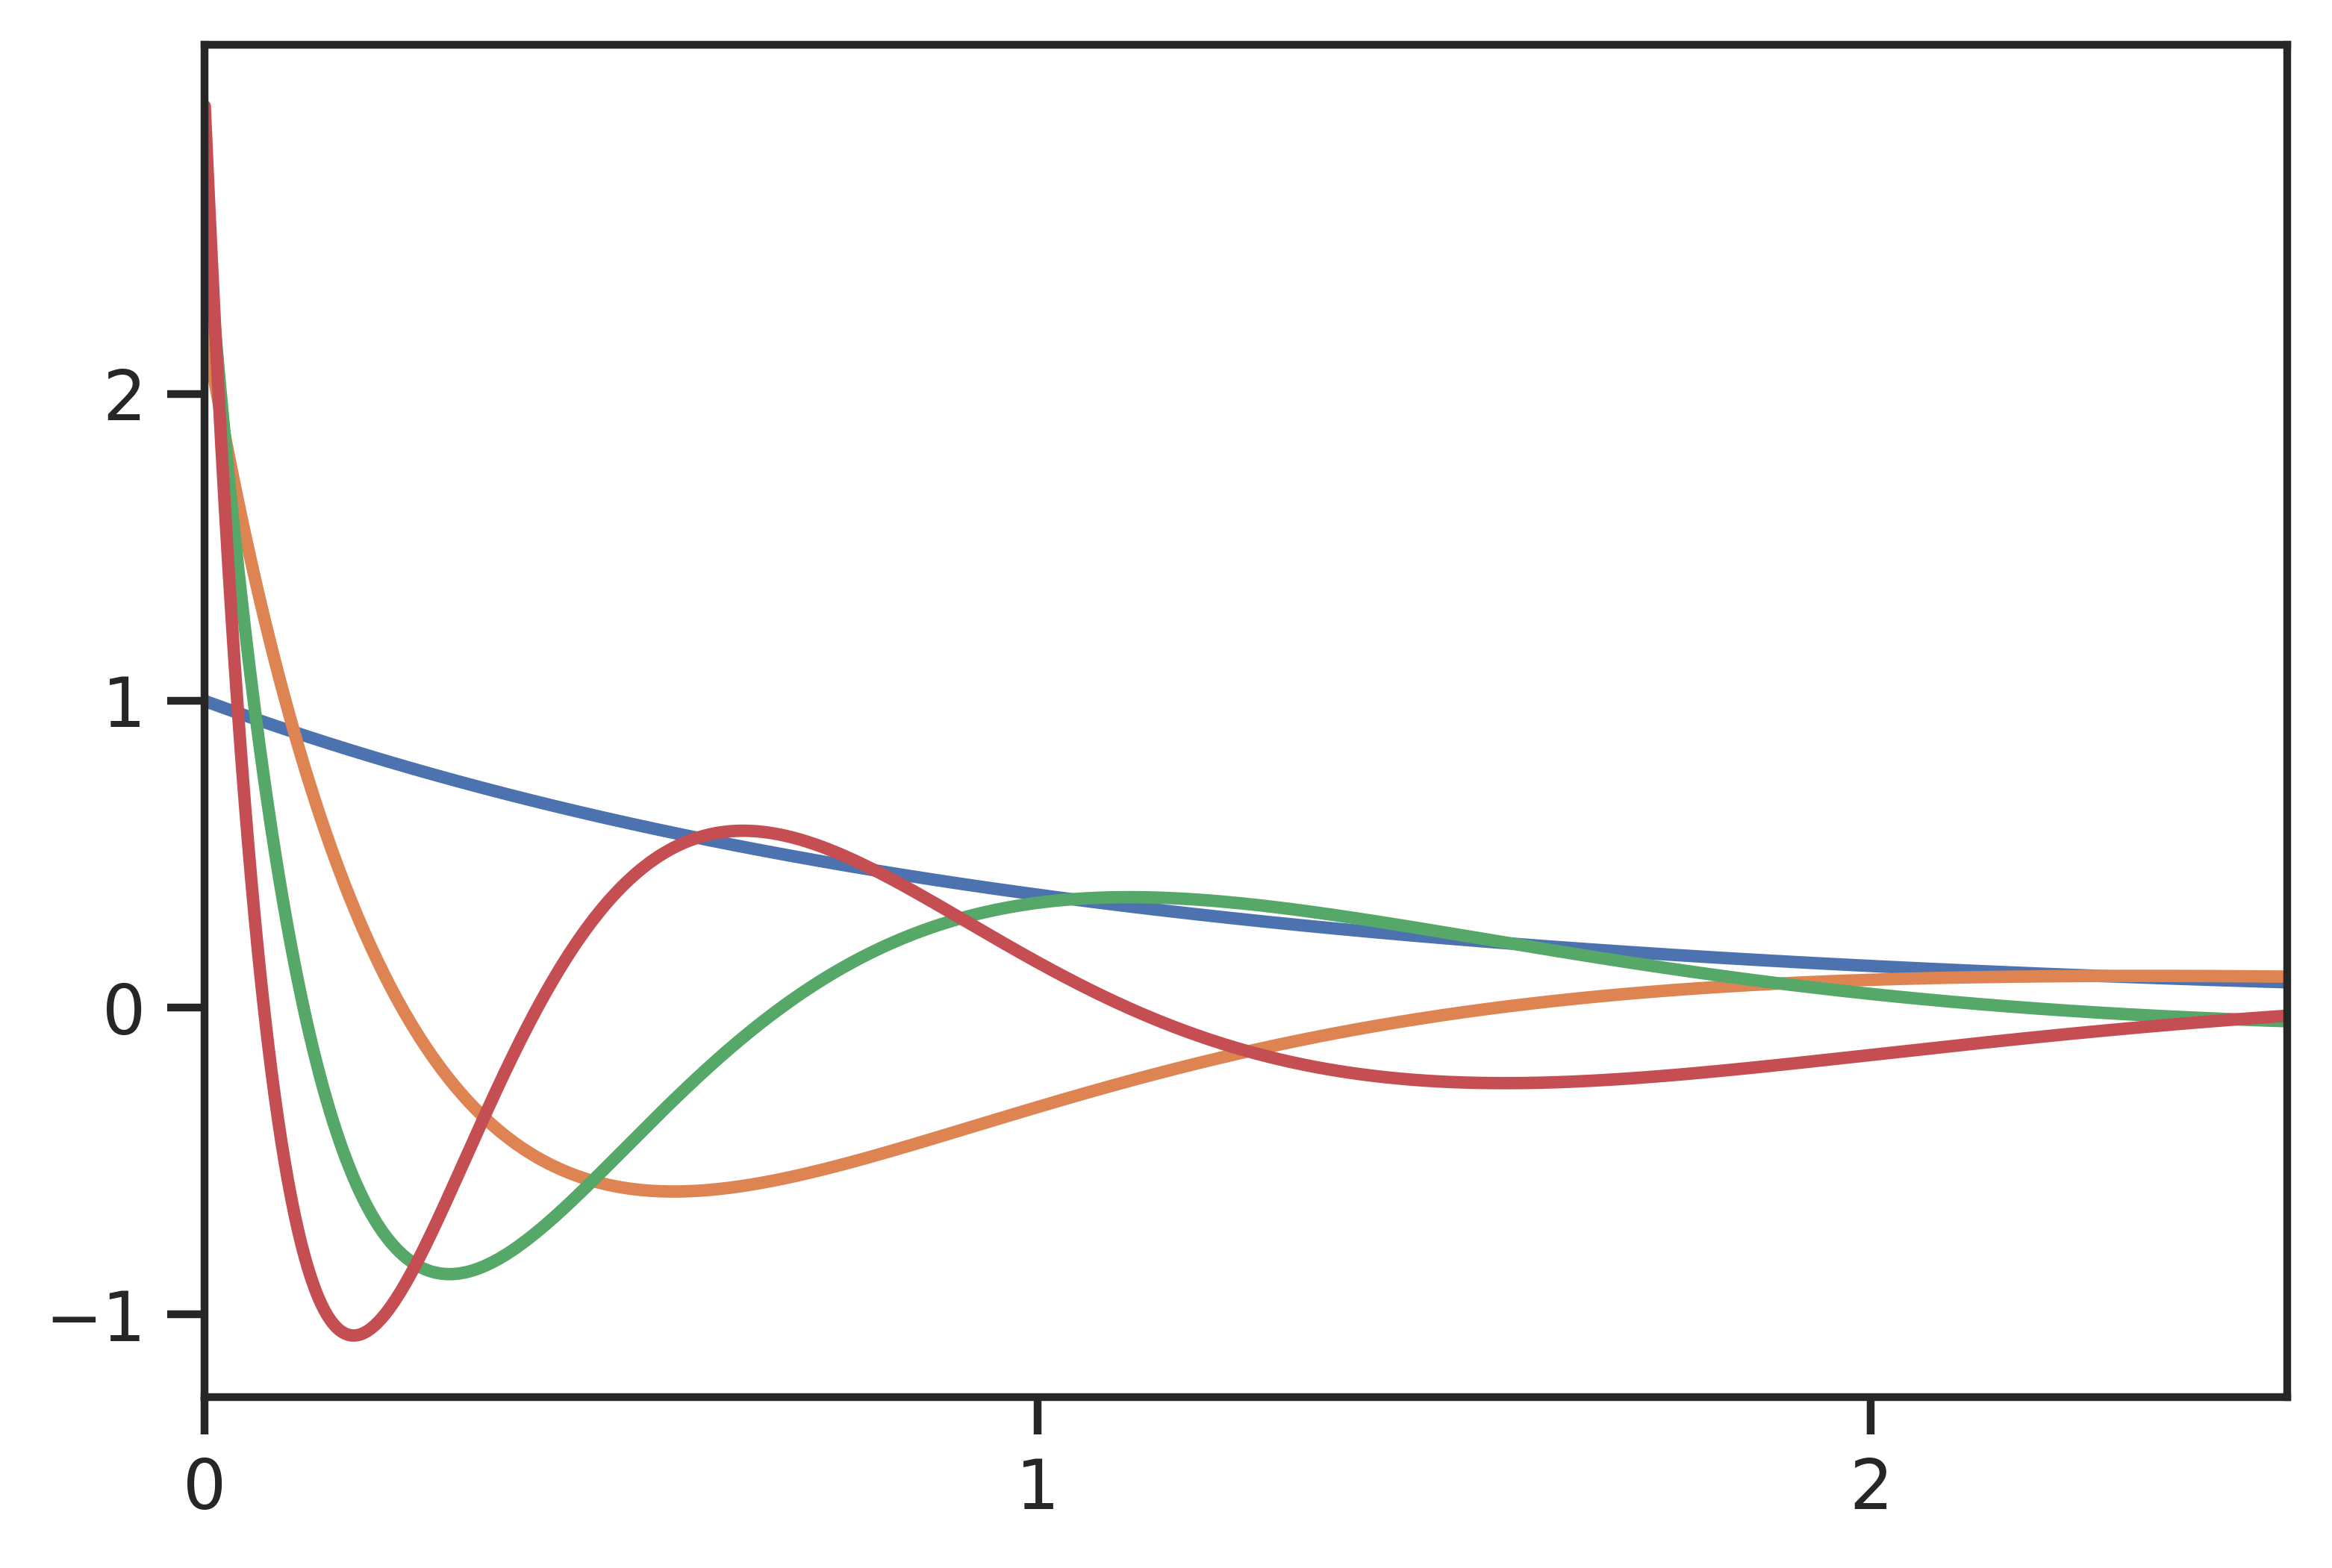
\includegraphics[width=0.5\textwidth]{Figs/hippo_kernel.png}
        
%         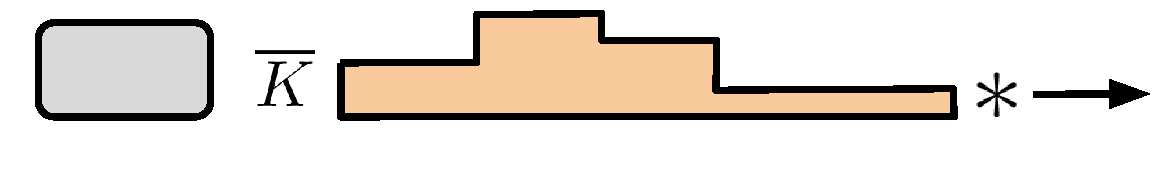
\includegraphics[width=0.5\textwidth]{Figs/SGParam.pdf}
%         \label{fig:enter-label}
%     \end{figure}
% \end{frame}

% \begin{frame}{S4 \cite{gu2022parameterization} }

% Learn parameters of SSM, convert to linear RNN parameters 

% $$\boldsymbol{\overline{A}}, \boldsymbol{\overline{B}}, \boldsymbol{\overline{C}}  = \text{discretize}(\boldsymbol{A}, \boldsymbol{B}, \boldsymbol{C}, \Delta )$$

%     \begin{figure}
%         \centering
%         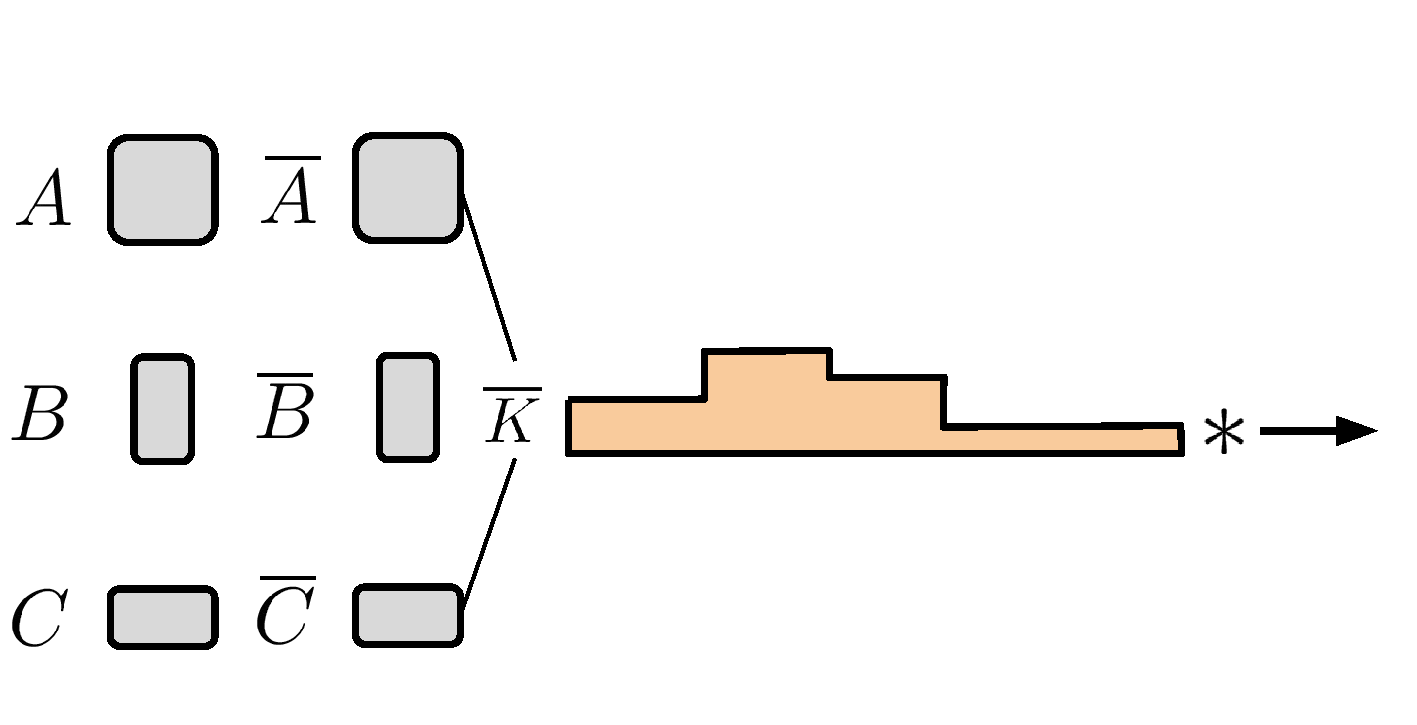
\includegraphics[width=0.6\textwidth]{Figs/SSMParam.pdf}
%         \caption{}
%         \label{fig:my_label}
%     \end{figure}
% \pause
% \vspace{-2cm}

% Note: There are \textit{many more} important details here.
    
% \end{frame}


% \begin{frame}{Determining RNN Parameterization}
% \begin{itemize}
% \item \cite{gu2020hippo} develop \textit{HiPPO} Matrix for SSM $\boldsymbol{A}$   

% % \begin{scriptsize}
% % \begin{align*}  
% % \boldsymbol{A}_{nk}= -
% % \begin{cases} 
% % (2n+1)^{1/2}(2k+1)^{1/2} & \text{if } n > k \\ n+1 &\text{if } n=k \text{\ else\ } 0
% % \end{cases} 
% % \end{align*}
% % \end{scriptsize}

%     \item Approximates history through Legendre coefficients 
% \end{itemize}
% \begin{figure}
%     \centering
%     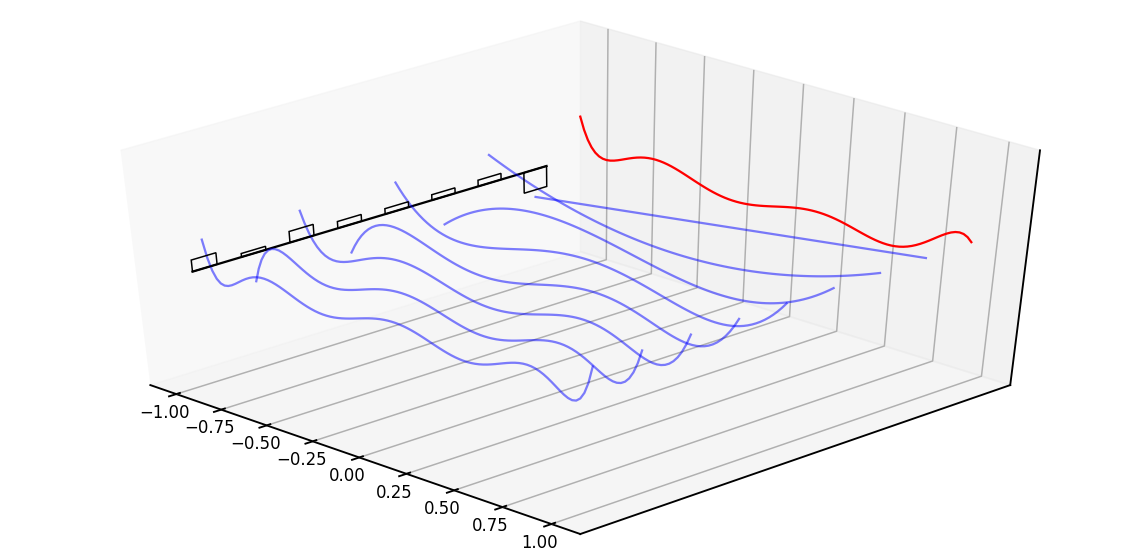
\includegraphics[width=0.7\textwidth]{Figs/hippo.png}
% \end{figure}
% \end{frame}

% \begin{frame}{Key Insight: Choice of $\boldsymbol{A}$ }

% \cite{gu2020hippo,gu2022parameterization}

% Show that HiPPO


% \end{frame}

\begin{frame}[c]{Results: ListOps \cite{gu2022parameterization}}
    \centering
        Example: [ $\uparrow$ 2 9 [ $\downarrow$ 4 7 ] 0 ] \textcolor{red}{9}
        
    \begin{figure}
        \centering

    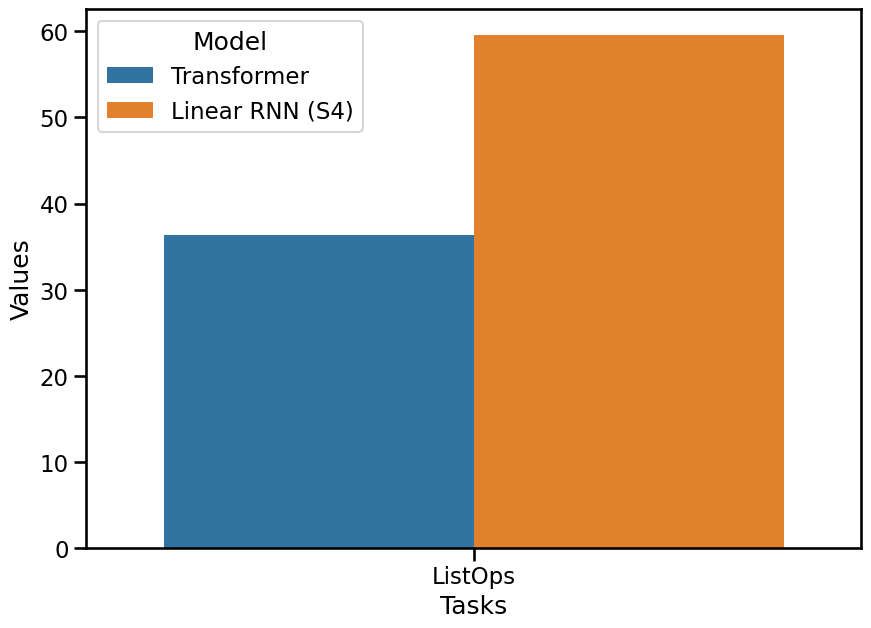
\includegraphics[height=0.6\textheight,clip,trim={0.1cm 0.1cm 0.1cm 0.1cm}]{Figs/listops-s4.png}
        \label{fig:my_label}
    \end{figure}
    Requires communication over 2,000  steps
    
\end{frame}


\begin{frame}[c]{Results: Long-Range Arena \cite{gu2022parameterization}}
    \centering
    \begin{figure}
        \centering
        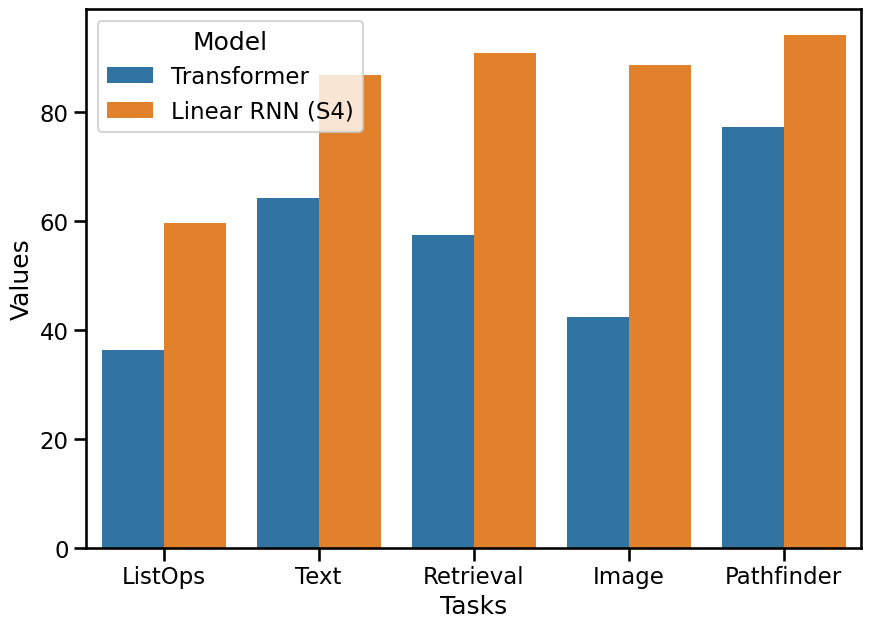
\includegraphics[height=0.8\textheight,clip,trim={0.1cm 0.1cm 0.1cm 0.1cm}]{Figs/lra-s4.png}
        \label{fig:my_label}
    \end{figure}
\end{frame}





% \begin{frame}{Computing with Static Kernels}
%     \structure{Final:} a b c $\Rightarrow$ d e f \textcolor{red}{d}

%     \begin{figure}
%         \centering
%         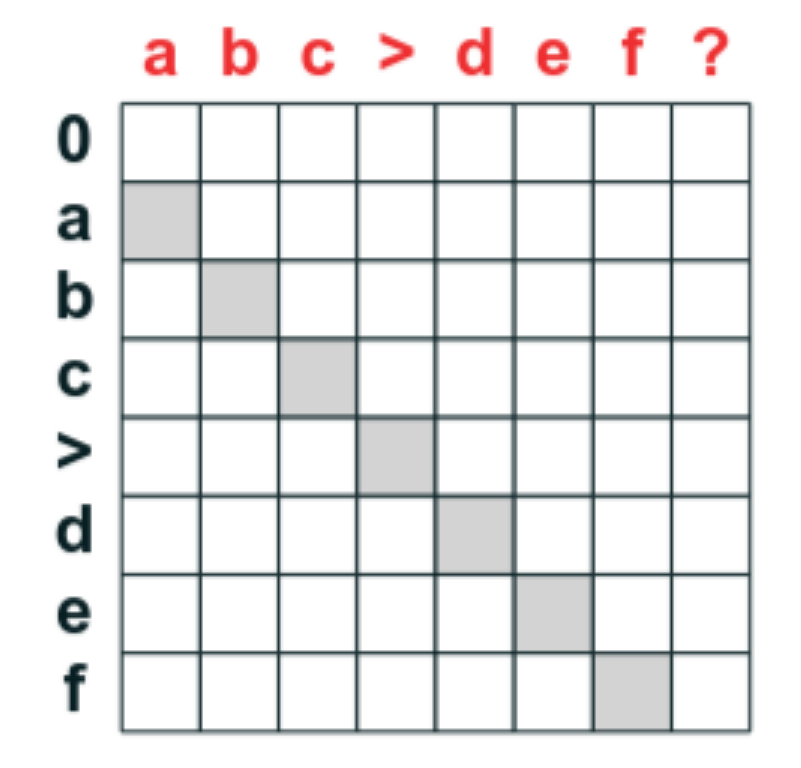
\includegraphics[height=0.5\textheight]{Figs/induct1.png}
%         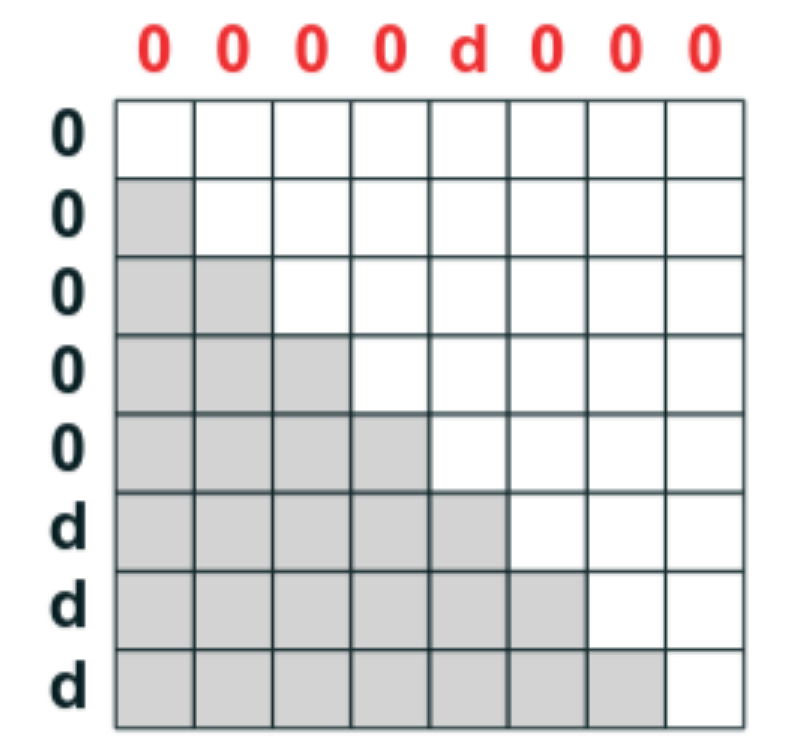
\includegraphics[height=0.5\textheight]{Figs/induct2.png}
%         \label{fig:my_label}
%     \end{figure}        
    
% \textcolor{blue}{Input:} a b c $\Rightarrow$ d e f \textcolor{red}{?}
 

% \end{frame}